%!TEX root = ../../main.tex

\chapter{Ist-Analyse}\label{ch:istanalyse}
In diesem Kapitel wird der Status quo bezüglich des automatisierten Testens bei FNT analysiert und dargestellt. Es wird dabei ein besonderer Fokus auf das Projekt \enquote{CIF Automated Tests} gelegt, da das in Kapitel \ref{ch:sollzustand} dieser Arbeit erarbeitete Konzept zur automatischen Testdatengenerierung auf diesem Projekt basiert.

\section{Automatisiertes Testen bei FNT}\label{sec:autotestsfnt}
Das automatisierte Testen stellt einen wichtigen Teil des allgemeinen Testprozesses bei \textit{FNT} dar. In vielen Softwareprojekten des Unternehmens kommen umfangreiche dedizierte Testprojekte mit automatisierten Testpipelines zusätzlich zum manuellen Testen zum Einsatz. Diese Testprojekte folgen alle der von der \textit{FNT} \ac{QA}-\ac{CoP} formulierten Testpolitik und Teststrategie, welche Anforderungen und Richtlinien zum Testen bei \textit{FNT} vorgeben und für alle Mitarbeiter*innen einsehbar sind. \cite{fnt:2020} \cite{fntstrat:2021}

Die automatisierten Tests bei \textit{FNT} verfolgen die Herangehensweise der \ac{CI}, um dem Prinzip der agilen Softwareentwicklung gerecht zu werden. \cite{fntstrat:2021} Hierbei wird eine längere Kette von Tests in verschiedenen Testphasen so häufig wie möglich schon während des Programmierens von Features automatisiert ausgeführt. Diese Testphasen oder auch Testsuites entsprechen dabei dem Konzept der Testpyramide, welche bereits in Kapitel \ref{subsec:testkonzepte} dargestellt wurde. \cite{fntstrat:2021} Die meisten Tests werden hierbei als \ac{E2E}-Tests realisiert.

Automatisierte Tests werden über eine \textit{Jenkins}-Pipeline, die \textit{QA-Build-Pipeline}, gestartet. Das Ausführen der einzelnen den Stufen der Testpyramide entsprechenden Testsuites in der Pipeline erfolgt über das Build-Automations-Tool \textit{Gradle} durch sogenannte \enquote{Tasks}. \textit{Jenkins} orientiert sich an einer \textit{build.gradle}-Datei, in welcher die Tasks definiert sind, und führt diese nacheinander automatisiert aus.

Der letzte Task in einer Testpipeline ist immer das Veröffentlichen eines Testreports in \textit{TestRail}. \textit{TestRail} ist eine Software zum Testmanagement, die es erlaubt, sowohl Testergebnisse als auch Testfälle ausführlich zu dokumentieren und zu verwalten. \cite{testrail:2022} \cite{fntstrat:2021}

Die regelmäßige Ausführung der automatisierten Tests über Build-Pipelines und die ausführliche Dokumentation von Testfällen und Testergebnissen sind wesentliche Faktoren, um eine hohe Testabdeckung und -qualität zu erreichen und zuverlässige Software von hoher Qualität zu produzieren, wie es in den Unternehmensrichtlinien als Ziel des Unternehmens definiert ist. \cite{fnt:2020}

\section{Das Projekt \enquote{CIF Automated Tests}}\label{sec:ciftestprojekt}
Das automatisierte Testen im Rahmen des Projekts \enquote{CIF Automated Tests} wurde im Jahr 2021 begonnen. Zuvor belief sich das Testen des \ac{CIF} ausschließlich auf manuell durchgeführte Tests, wodurch der Aufwand zum Testen des gesamten Systems sehr hoch und auch ein sehr häufiges und effizientes Testen wie in anderen bereits automatisierten Projekten nicht möglich war. Mit der Integration des \ac{CIF} in die Standardmodule von \textit{Command} bekommt dessen Zuverlässigkeit allerdings einen immer höheren Stellenwert, da das Modul so an eine deutlich größere Zahl von Kunden ausgeliefert wird. Fehler im \ac{CIF} könnten so zu einer Abwertung des gesamten Images der Software führen. Unter diesem Gesichtspunkt soll mithilfe von automatisierten Tests eine Steigerung der Sicherheit und Qualität des \ac{CIF} erreicht werden.

Das Testprojekt selbst richtet sich nach den in Kapitel \ref{sec:autotestsfnt} erwähnten vorgegebenen Richtlinien zum automatisierten Testen bei FNT. Getestet wird in zehn verschiedenen Testsuites, welche durch \textit{Gradle}-Tasks in der Build-Pipeline ausführbar sind. Die Testsuites sind im Folgenden aufgelistet. 

\begin{enumerate}
    \item \textbf{Suite \enquote{apiCommandAlive}}: Es wird ein schneller Check durchgeführt, um zu überprüfen, ob die zu testenden \textit{Command}-Instanz erreichbar ist. Schlägt dieser Check fehl, so wird der Build sofort abgebrochen, da die Erreichbarkeit der Instanz eine Voraussetzung zur Durchführung aller weiteren Tests ist.
    \item \textbf{Suite \enquote{apiPreconditions}}: In der Precondition-Suite werden einige für die weiteren Tests benötigte Objekte in \textit{Command} angelegt. Dies beinhaltet beispielsweise einen Job, welcher zur Steuerung des Datenintegrationsprozesses nötig ist, und eine Zone, das heißt ein virtueller Campus mit einem Gebäude, einer Etage und einem Raum. Diese Zone muss für spätere Tests vorhanden sein, um Geräte darin platzieren zu können.
    \item \textbf{Suite \enquote{apiSmoke}}: Die Smoke-Suite besteht aus Tests, welche grundlegende Funktionen von \textit{Command} beziehungsweise des \ac{CIF} auf korrekte Funktionalität prüfen. Hierzu gehört sowohl das ausgiebige Testen der Login-Funktion als auch ein erster Check, ob die Deltaberechnung grundsätzlich durchführbar ist. Schlagen Tests in der Smoke-Suite fehl, wird der Build sofort abgebrochen, da bei Fehlern in diesen grundlegenden Funktionen ein weiteres Testen von Komponenten, die oft auf diesen Funktionen basieren, sinnlos wäre.
    \item \textbf{Suite \enquote{apiSetUpEnvironment}}: In dieser Suite wird eine Testumgebung für die darauffolgenden \ac{E2E}-Tests geschaffen. Mithilfe von vordefinierten Testdaten werden Testobjekte so in \textit{Command} und in die \ac{NMS}-Tabelle platziert, dass alle möglichen Deltafälle berechnet werden und in den weiteren Tests getestet werden können.
    \item \textbf{Suite \enquote{apiRegression}}: In der Regression-Suite werden Integrationstests ausgeführt. Hierzu zählt beispielsweise das Erstellen von einzelnen Objekten in der \ac{NMS}-Tabelle.
    \item \textbf{Suite \enquote{apiRegressionE2E}}: Diese Suite beinhaltet funktionale \ac{E2E}-Tests. Getestet wird hierbei, ob die Deltafälle korrekt berechnet wurden, ob die Deltas genehmigt werden können und in \textit{Command} korrekt synchronisiert werden. Aufgrund der hohen Anzahl von Tests in dieser Suite wurde sie in einzelne Komponenten aufgeteilt:
    \begin{description}
        \item[Hardware:] Diese Tests betrefen alle möglichen Hardware-Entitäten, beispielsweise Chassis oder Modules.
        \item[Zone:] Die Zonentests betreffen alle Arten von Zonen, zum Beispiel Buildings oder Rooms.
    \end{description}
    \item \textbf{Suite \enquote{uiRegression}}: Diese Suite dient zum Durchführen grundlegender Tests über die \ac{GUI} von \textit{Command}, sodass deren Funktionalität geprüft werden kann.
    \item \textbf{Suite \enquote{uiRegressionE2E}}: In der UI-\ac{E2E}-Suite werden \ac{E2E}-Tests über die \ac{GUI} durchgeführt. Ganze Funktionsketten werden über \ac{GUI}-Interaktionen ausgeführt und getestet.
    \item \textbf{Suite \enquote{apiCleanEnvironment}}: Diese Suite dient zur Überprüfung, ob Objekte aus \textit{Command} auch wieder gelöscht werden können und bereinigt gleichzeitig die zu testende Instanz von allen bei der Testdurchführung erstellten Testobjekten.
    \item \textbf{Task \enquote{publishReportToTestRail}}: Der letzte Task bei der Testausführung ist kein Testtask. Stattdessen werden die Ergebnisse des Testlaufs an \textit{TestRail} übermittelt, wo sie grafisch aufbereitet einsehbar sind.
\end{enumerate}

Wie in den aufgeführten Tasks zu erkennen, wird eine Unterscheidung zwischen \ac{API}- und \ac{GUI}-Tests vorgenommen. \ac{API}-Tests führen all die in \textit{Command} zu testenden Funktionen über die \textit{Command}-\ac{API}, die \ac{BGE}s, aus. \ac{GUI}-Tests \enquote{klicken} hingegen zur Ausführung der zu testenden Funktionen mithilfe von Tools wie \textit{Selenium} tatsächlich auf Elemente der grafischen Oberfläche von \textit{Command}, wie es ein Benutzer der Software tun würde. Sie sind dementsprechen aber auch sehr langsam und aufwendig zu implementieren, weshalb deutlich mehr \ac{API}-Tests realisiert werden.

Die Tasks werden in der \textit{build.gradle}-Datei definiert und in einer auf \textit{Groovy} basierenden Skriptsprache geschrieben. Das folgende Codebeispiel zeigt einen beispielhaften Task zum Ausführen der \ac{API}-\ac{E2E}-Testsuite. Schlägt dort ein Test fehl, wird dies dokumentiert und am Ende des Testlaufs ein Fehlerreport an \textit{TestRail} übermittelt.

\begin{lstlisting}[caption=Ein Beispiel eines Gradle Tasks zum Ausführen einer Testsuite, label=Gradle-Task-Code, language=Groovy]
task apiHardwareRegressionE2E(type: Test) {
    description = 'Run api hardware regression tests with annotation @Tag(suite:regressionApiE2E)'
    group = 'testing'
    
    useJUnitPlatform() {
        includeTags 'suite:regressionApiE2E'
        ignoreFailures false
    }
    filter {
        includeTestsMatching "*com.fntsoftware.api.CommandApiHardwareE2ETests*"
    }
}
\end{lstlisting}

Die Tests werden in Java implementiert und über die Java-Testplattform \textit{JUnit} ausgeführt. \textit{JUnit} erlaubt das Verwenden von Annotationen an den einzelnen Tests, beispielsweise um diese einfach in Testsuites zu gruppieren. Gerade diese Annotation kann in den Gradle Tasks genutzt werden, um wie in Listing \ref{Gradle-Task-Code} alle vorhandenen Tests zu filtern und nur die Tests einer bestimmten Testsuite auszuführen. \cite{junit:2021}

\begin{lstlisting}[caption=Ein Test in JUnit mit Annotationen, label=JUnit-Test,style=Javastyle]
@Tag("suite:regressionApiE2E")
@Test
void C19640285_VerifyThatChassisWillBeCreatedInCommandE2E() throws IOException, InterruptedException {
	BgeQueryResponse<DeltaTableResponse> deltaTableResponse = deltaStep.queryDeltaReportHardware(this.sessionId, "Chassis", "TEST_CHASSIS_CREATE");
	Assertions.assertEquals("CREATE", deltaTableResponse.getReturnData().get(0).getDeltaCase());

	// Set data approved
	deltaStep.setDeltaApproved(this.sessionId, deltaTableResponse.getReturnData().get(0).getHashElid());

	// Synchonization
	BgeQueryResponse<BgeRunInterfaceResponse> syncResponse = interfaceStep.executeJobSync(this.sessionId, "SYNCHRONIZE");
	Assertions.assertEquals("FINISHED", syncResponse.getReturnData().get(0).getStatus());

	// Verify Data
	Assertions.assertFalse(cmdBgeApiStep.querySpecificCommandObjects(this.sessionId, "TEST_CHASSIS_CREATE", "chassis", CommandChassisModel.class).isEmpty(), "Chassis has been created succesfully");
}
\end{lstlisting}

\section{Testdaten im Projekt \enquote{CIF Automated Tests}}\label{sec:testdatenIst}
Das Projekt \enquote{CIF Automated Tests} arbeitet, wie die meisten anderen Testprojekte bei \textit{FNT}, mit statischen Testdaten in \ac{JSON}-Dateien. Diese werden von Hand manuell erstellt und gepflegt. In den einzelnen \ac{JSON}-Dateien werden die Daten in Form eines Arrays gehalten, wobei ein Arrayeintrag ein Testdatenobjekt darstellt. Für jede Entität existieren mehrere \ac{JSON}-Dateien, um die bereits in Kapitel \ref{sec:deltacases} angesprochenen Anforderungen an die Deltafälle abzudecken - die Testdatenobjekte, welche in die verschiedenen Tabellen in \textit{Command} platziert werden müssen, lassen sich so besser gruppieren. In der folgenden Abbildung ist ein Beispiel für die Verwendung manueller Testdatendateien für die Entität Chassis dargestellt.

\begin{figure}[h]
    \centering
    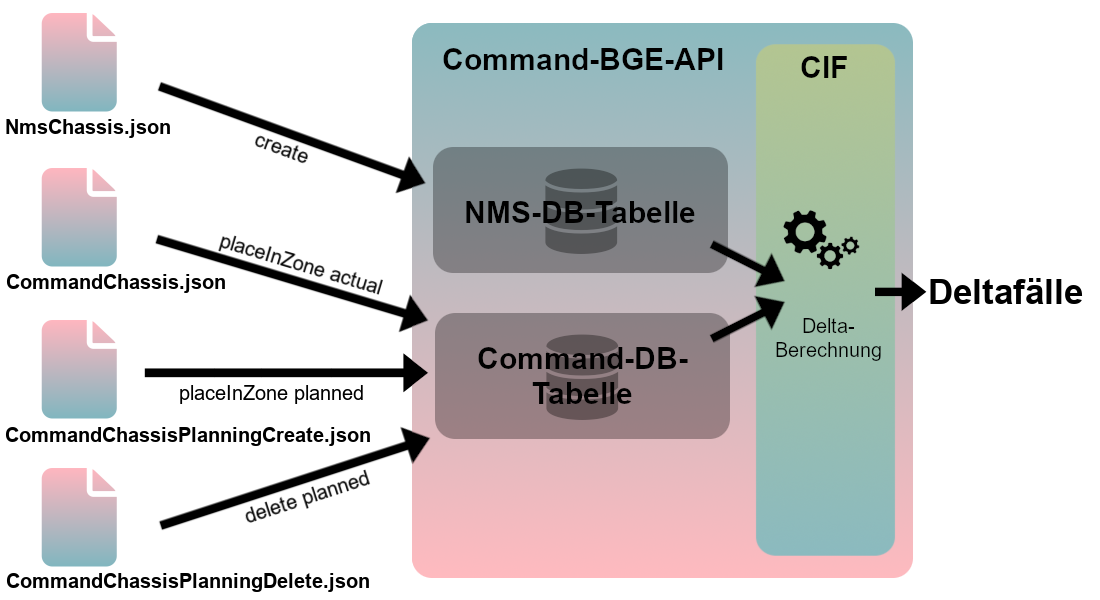
\includegraphics[width=.8\textwidth]{manual-testdata-import.png}
    \caption{Verwendung manueller Testdatendateien}
\end{figure}

Im Folgenden ist ein Objekt der Entität Chassis beispielhaft in \ac{JSON}-Form angegeben, wie es in einer der Testdatendateien vorkommen kann.

\begin{lstlisting}[caption=Testdaten für ein Chassis in JSON-Form, label=JSON-Testdaten,language=json]
[
    {
        "cSourceId": "TEST_CHASSIS_UPDATE",
        "selectedSourceSystem": "CIF_AUTOMATED_TEST",
        "cSourceType": "OSN2500",
        "id": "TEST_CHASSIS_UPDATE",
        "sourceSystem": "CIF_AUTOMATED_TEST",
        "visibleId": "TEST_CHASSIS_UPDATE",
        "ipAddress": "10.122.77.02",
        "hwRevision": "HW Version6",
        "swRevision": "SW Version6",
        "remark": "C19640286: Test nms chassis UPDATE",
        "serialNo": "123456561",
        "createLinkDeviceMaster": {
          "linkedElid": "EKJAG5VN1YBKEH"
        },
        "createLinkZone": {
          "linkedElid": "7RJHP3VXHV4VJO"
        }
    }
]
\end{lstlisting}

Die \ac{JSON}-Dateien werden in der Testsuite \textit{apiSetUpEnvironment} zunächst geparst und die einzelnen Arrayeinträge mithilfe der Java Bibliothek \textit{Jackson} zu Objekten von sogenannten \ac{POJO}-Klassen deserialisiert. Daraufhin muss bei jedem Objekt einzeln der Wert für die \ac{Elid} der verlinkten Zone abgeändert werden. Dies hat den Grund, dass die Zone, in welcher während eines Testlaufs Testobjekte platziert werden, nach jedem Testlauf gelöscht und daher immer wieder neu erstellt werden muss. Hierbei verändert sich auch immer die \ac{Elid} der Zone, da \ac{Elid}s einzigartig sind und für jedes neu erstellte Objekt in \textit{Command} generiert werden. Dieser Wert kann also nur zur Zeit der Testausführung korrekt gesetzt werden.

Sind für alle Objekte die Attribute mit korrekten Werten gefüllt, werden sie über Aufrufe von dafür vorgesehenen \ac{REST}-Endpunkten der \ac{BGE}s entweder in die \ac{NMS}-Tabellen gefüllt oder in \textit{Command} erstellt beziehungsweise gelöscht.

\section{Implementierung von Testfällen}\label{sec:testimplementierung}
Ein Projekt in einer unbekannten Softwareumgebung wie dem \ac{CIF} und insbesondere den damit verbundenen automatisierten Tests zu realisieren ist nicht einfach. Die Gefahr besteht, dass aufgrund von mangelndem Know-How wichtige Funktionalitäten übersehen oder mögliche Vorgehensweisen nicht eingesetzt werden, welche das Projekt effektiver umsetzbar machen könnten. Zur Vermeidung dessen wurde noch vor einer ersten Konzeptionierung der geplanten automatischen Testdatengenerierung eine Einarbeitung in das \ac{CIF} und das Projekt \enquote{CIF Automated Tests} vorgenommen, indem noch nicht realisierte Testfälle implementiert werden sollten.

Es stellte sich dabei heraus, dass das Implementieren der eigentlichen Tests die wenigste Zeit in Anspruch nahm. Die größte Hürde stellten die Testdaten dar, welche manuell erstellt werden mussten. Gerade Entitäten, mit welchen sich zuvor nicht beschäftigt wurde, stellten eine Herausforderung dar. Es war unklar, welche Informationen die Testdaten beinhalten mussten und welche Werte für bestimmte Attribute gewählt werden sollten. Dies führte zu vielen fehlgeschlagenen Tests, da immer wieder Fehler in der Konfiguration der Testdaten gemacht wurden.

Selbst wenn die Testdaten korrekt formuliert waren, konnten sie auf anderen \textit{Command}-Versionen fehlschlagen, da dort einige der in den Testdatendateien festgelegten Gerätetypen gar nicht existierten. Hierbei offenbart sich ein großer Nachteil in der Herangehensweise der manuell erstellten und in externen Dateien gespeicherten Testdaten: Sie sind unflexibel und damit kaum portabel. 

Portabilität im Software-Rahmen bedeutet, dass Software auf anderen Systemen ausgeführt werden kann als auf dem, für das sie ursprünglich geschrieben wurde. \cite{brown:2003} Angewandt auf den Kontext der Softwaretests sollen portable Tests also auf verschiedenen \ac{SUT}s erfolgreich ausgeführt werden können. Beim Testen des \ac{CIF} hat dies eine große Wichtigkeit, da Kunden nach wie vor ältere Versionen des Moduls verwenden, die weiterhin getestet werden müssen. Die automatisierten Tests sollen also ohne großen weiteren Aufwand auch auf anderen \ac{CIF}- beziehungsweise \textit{Command}-Versionen ausführbar sein und zuverlässige Ergebnisse liefern. Statische \ac{JSON}-Dateien sind jedoch speziell auf die \textit{Command}-Instanz angepasst, für die sie erstellt wurden, und können nur mit größeren Änderungen für andere Instanzen verwendet werden. 

Die Implementierung der Testfälle diente also nicht nur zur Einarbeitung in die Testumgebung, sondern konnte auch bestätigen, weshalb eine automatische Testdatengenerierung überhaupt implementiert werden sollte. Automatisch generierte Testdaten können die Portabilität von Tests erheblich verbessern, wie auch anonym befragte Tester*innen bei \textit{FNT} bestätigen. (s. Anhang \nameref{app:befragung}, Frage 13)